%%%%%%%%%%%%%%%%%%%%%%%%%%%%%%%%%%%%%%%%%%%%%%%%%%%%%%%%%%%%%%%%
%%%%%%%%%%%%%%%%%%%%%%%%%%%%%%%%%%%%%%%%%%%%%%%%%%%%%%%%%%%%%%%%
%%%%
%%%% This text file is part of the source of 
%%%% `Introduction to High-Performance Scientific Computing'
%%%% by Victor Eijkhout, copyright 2012-8
%%%%
%%%% This book is distributed under a Creative Commons Attribution 3.0
%%%% Unported (CC BY 3.0) license and made possible by funding from
%%%% The Saylor Foundation \url{http://www.saylor.org}.
%%%%
%%%%
%%%%%%%%%%%%%%%%%%%%%%%%%%%%%%%%%%%%%%%%%%%%%%%%%%%%%%%%%%%%%%%%
%%%%%%%%%%%%%%%%%%%%%%%%%%%%%%%%%%%%%%%%%%%%%%%%%%%%%%%%%%%%%%%%

A \indexacf{GPU} (or sometimes \indexacf{GPGPU}) is a special purpose processor,
designed for fast graphics processing. However, since the operations
done for graphics are a form of arithmetic, \acp{GPU} have gradually
evolved a design that is also useful for non-graphics computing.
The general design of a \ac{GPU} is motivated by the `graphics
pipeline': identical
operations are performed on many data elements
in a form of \indexterm{data parallelism}
(section~\ref{sec:data-parallel}),
and a number of such
blocks of data parallelism can be active at the same time.

\begin{wrapfigure}{r}{3.5in}
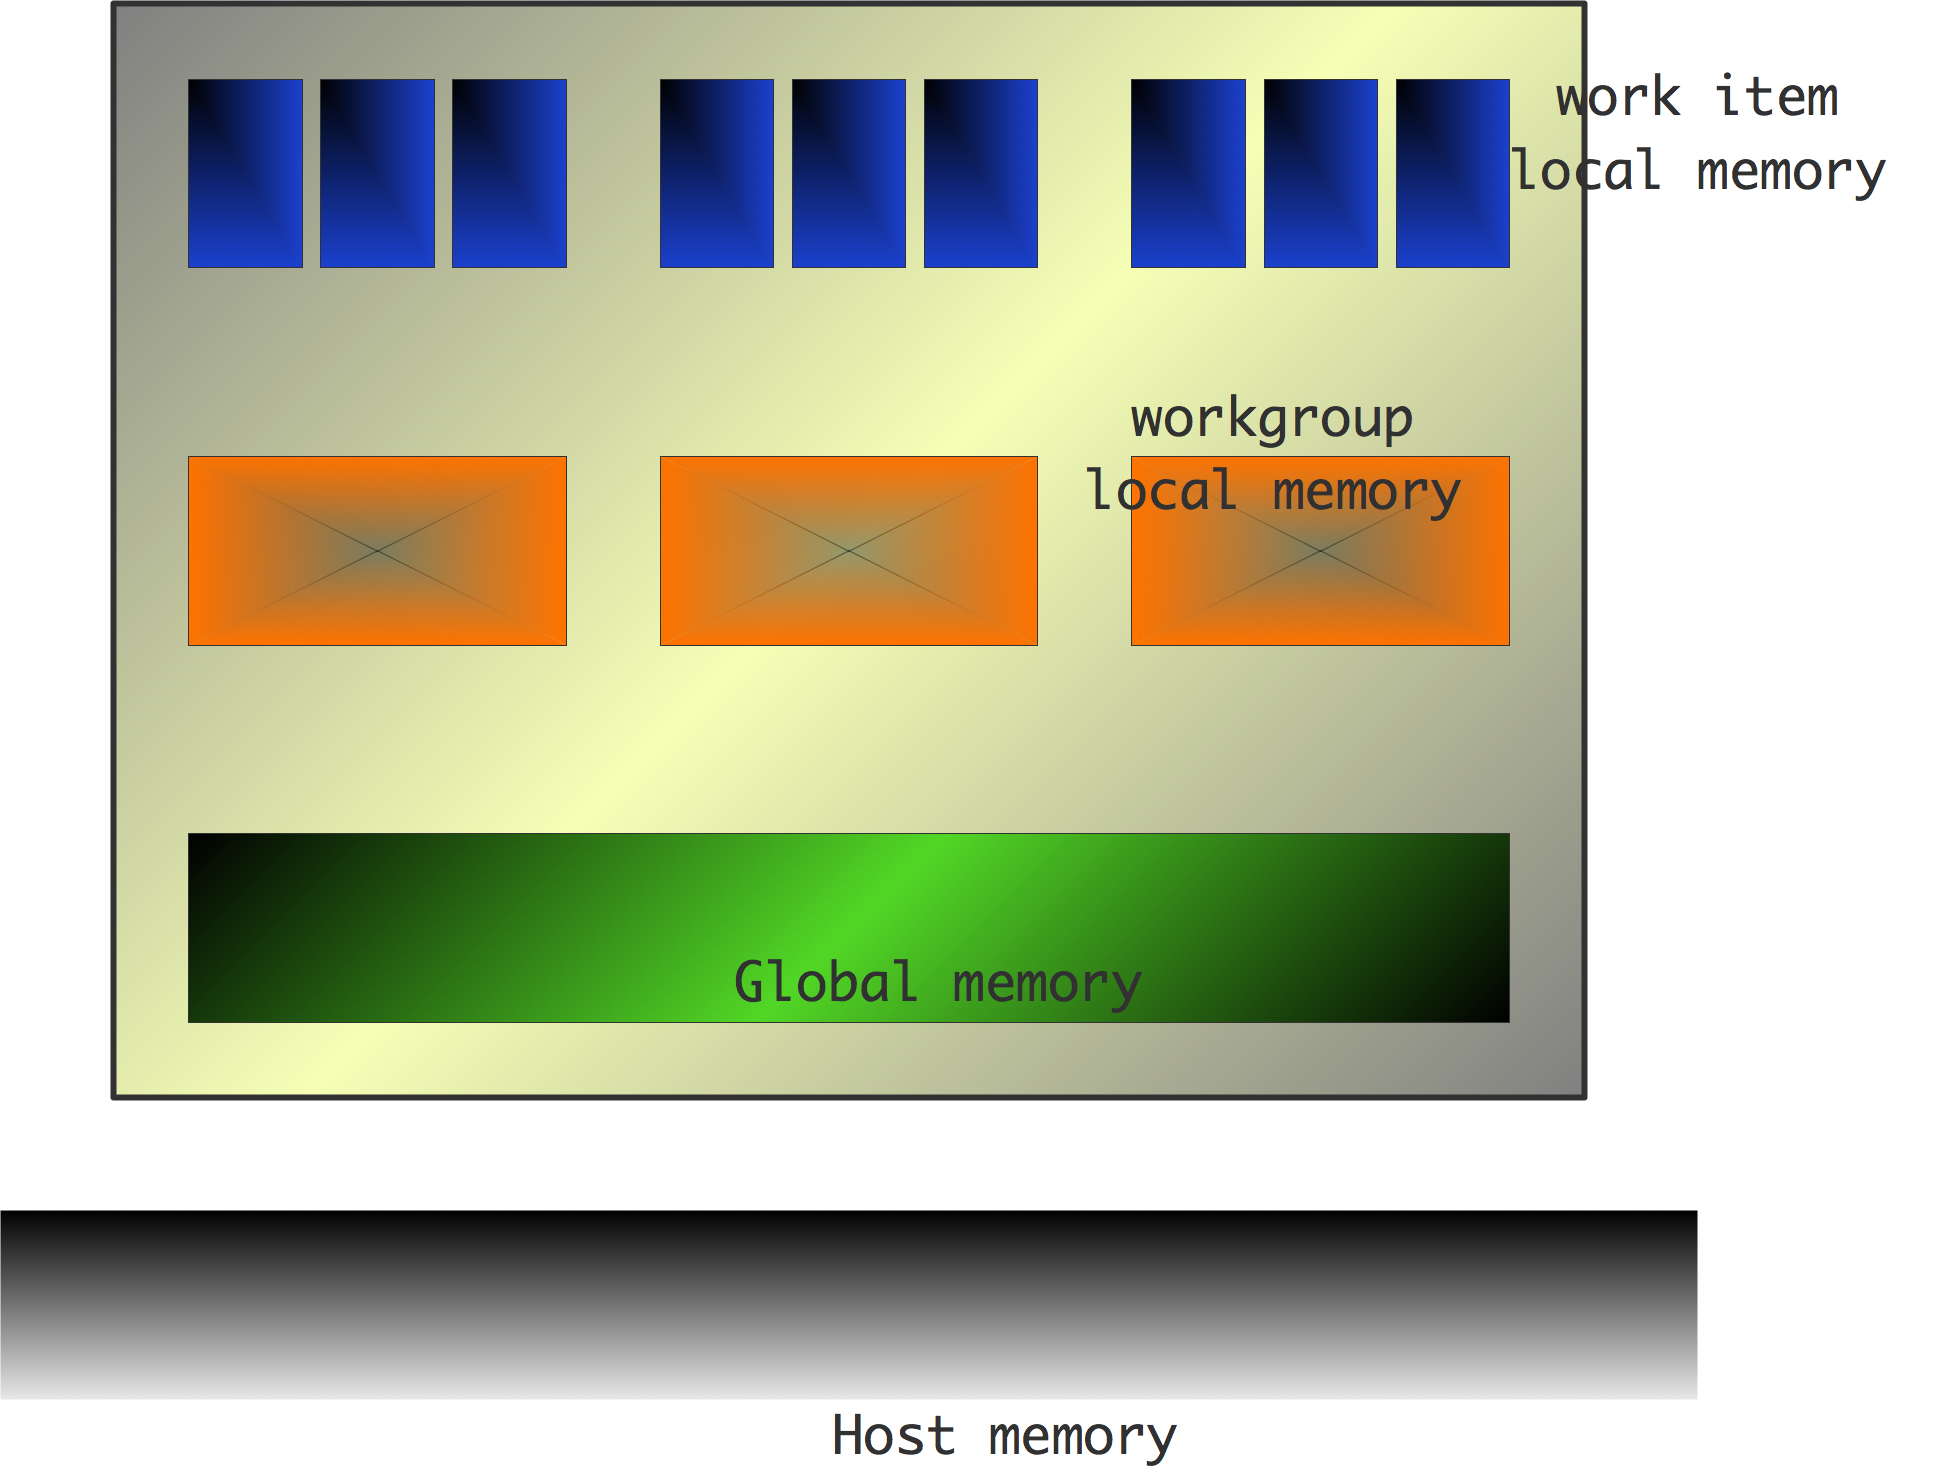
\includegraphics[scale=.15]{gpu-memory}
\caption{Memory structure of a GPU}
\label{fig:gpu-memory}
\end{wrapfigure}
%
The basic limitations that hold for a CPU hold for a \ac{GPU}:
accesses to memory incur a long latency. The solution to this problem
in a CPU is to introduce levels of cache; in the case of a \ac{GPU} a
different approach is taken (see also
section~\ref{sec:mta}). \acp{GPU} are concerned with
\indexterm{throughput computing}, delivering large amounts of data
with high average rates, rather than any single result as quickly as
possible. This is made possible by supporting many threads
(section~\ref{sec:threads}) and having very fast switching between
them. While one thread is waiting for data from memory, another thread
that already has its data can proceed with its computations.

\Level 2 {SIMD-type programming with kernels}
\label{sec:gpu-kernel}

Present day \acp{GPU}
\begin{footnoteenv}
{The most popular GPUs today are made by
  NVidia, and are programmed in \indexterm{CUDA}, an extension of the
  C language.}
  \end{footnoteenv}
have an architecture that combines \ac{SIMD}
and \ac{SPMD} parallelism. Threads are not completely independent, but
are ordered in \indextermbus{thread}{blocks}, where all threads in the
block execute the same instruction, making the execution \ac{SIMD}. It
is also possible to schedule the same instruction stream
(a~`kernel'\index{kernel!CUDA} in Cuda terminology) on more than one
thread block. In this case, thread blocks can be out of sync, much
like processes in an \ac{SPMD} context. However, since we are dealing
with threads here, rather than processes, the term \indexac{SIMT} is used.

This software design is apparent in the hardware; for instance, an
NVidia \ac{GPU} has 16--30 \acfp{SM}, and a \acp{SM} consists of 8
\acfp{SP}, which correspond to processor cores; see
figure~\ref{fig:gpu-diagram}. The \acp{SP} act in true SIMD fashion.
The number of cores in a \ac{GPU} is
typically larger than in traditional multi-core processors, but the
cores are more limited. Hence, the term \indexterm{manycore} is used here.

\begin{figure}[ht]
  \begin{quote}
    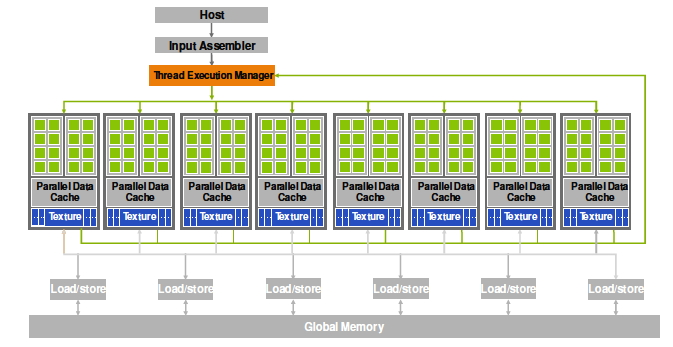
\includegraphics[scale=.6]{graphics/gpu1}
  \end{quote}
  \caption{Diagram of a GPU}
  \label{fig:gpu-diagram}
\end{figure}

The \ac{SIMD}, or \indexterm{data parallel}, nature of \acp{GPU} becomes
apparent in the way \indexterm{CUDA} starts
processes. A~\emph{kernel}\index{kernel!CUDA}, that is, a function that will
be executed on the \ac{GPU}, is started on $mn$ cores by:
\begin{verbatim}
KernelProc<< m,n >>(args)
\end{verbatim}
The collection of $mn$ cores executing the kernel is known as a
\emph{grid}\index{grid (CUDA)}, and it is structured as
$m$~\indextermbus{thread}{blocks} of $n$~threads each. 
A~thread block can have up to 512 threads.

Recall that threads share an address space (see
section~\ref{sec:threads}), so they need a way to identify what part
of the data each thread will operate on. For this, the blocks in a
thread are numbered with $x,y$ coordinates, and the threads in a block
are numbered with $x,y,z$ coordinates. Each thread knows its
coordinates in the block, and its block's coordinates in the grid.

We illustrate this with a vector addition example:
\begin{verbatim}
// Each thread performs one addition
__global__ void vecAdd(float* A, float* B, float* C)
{
  int i = threadIdx.x + blockDim.x * blockIdx.x;
  C[i] = A[i] + B[i];
}
int main()
{
  // Run grid of N/256 blocks of 256 threads each
  vecAdd<<< N/256, 256>>>(d_A, d_B, d_C);
}
\end{verbatim}
This shows the \ac{SIMD} nature of \acp{GPU}: every thread executes
the same scalar program, just on different data.

\begin{comment}
\begin{quote}
\begin{tabular}{|c|cccc|}
  \hline
     & SM & SP & thread blocks    & threads\\ \hline
  GPU& 16 &    & $8\times 16=128$ & \\
  SM &    &  8 & 8                & 768 \\
  \hline
\end{tabular}
\end{quote}
\end{comment}


\begin{comment}
The total internal bandwidth is about 80 Gbyte or 10 Gword per second,
or 100 Mword per \ac{SP}.
By contrast, the bandwidth to main memory (over the \indexterm{PCI-X bus}) is only
4 Gbyte per second, each way.
\end{comment}

Threads in a thread block are truly data parallel: if there is a
conditional that makes some threads take the \emph{true} branch and
others the \emph{false} branch, then one branch will be executed
first, with all threads in the other branch stopped. Subsequently,
\emph{and not simultaneously}, the threads on the other branch will
then execute their code. This may induce a severe performance penalty.

\acp{GPU} rely on a large amount of data parallelism and the ability to
do a fast
\indextermbus{context}{switch}. This means that they will thrive in
graphics and scientific applications, where there is lots of data
parallelism. However they are unlikely to do well on `business
applications' and operating systems, where the parallelism is of the
\acf{ILP} type, which is usually limited.

\Level 2 {GPUs versus CPUs}

These are some of the  differences between \acp{GPU} and regular CPUs:
\begin{itemize}
\item First of all, as of this writing (late 2010), \acp{GPU} are
  attached processors, for instance over a \indexterm{PCI-X bus},
  so any data they operate on has to be
  transferred from the CPU. Since the memory \indexterm{bandwidth} of
  this transfer is low, at least 10 times lower than the memory
  bandwidth in the \ac{GPU}, sufficient work has to be done on the \ac{GPU}
  to overcome this overhead.
\item Since \acp{GPU} are graphics processors, they put an emphasis on
  \indexterm{single precision} floating point arithmetic. To
  accommodate the scientific computing community, \indexterm{double
    precision} support is increasing, but double precision speed is
  typically half the single precision flop rate. This discrepancy is
  likely to be addressed in future generations.
\item A CPU is optimized to handle a single stream of instructions
  that can be very heterogeneous in character; a~\ac{GPU} is made
  explicitly for data parallelism, and will perform badly on
  traditional codes.
\item A CPU is made to handle one \indexterm{thread}, or at best a
  small number of threads. A~\ac{GPU} \emph{needs} a large number of
  threads, far larger than the number of computational cores, to
  perform efficiently.
\end{itemize}

\Level 2 {Expected benefit from GPUs}

\acp{GPU} have rapidly gained a reputation for achieving high
performance, highly cost effectively. Stories abound of codes that
were ported with minimal effort to CUDA, with a resulting speedup of
sometimes $400$ times. Is the GPU really such a miracle machine? Were
the original codes badly programmed? Why don't we use GPUs for
everything if they are so great?

The truth has several aspects. 

First of all, a \ac{GPU} is not as general-purpose as a regular CPU:
\acp{GPU} are very good at doing \indexterm{data parallel} computing,
and CUDA is good at expressing this fine-grained parallelism
elegantly. In other words, \acp{GPU} are suitable for a certain type
of computation, and will be a poor fit for many others.

Conversely, a regular CPU is not necessarily good at data
parallelism. Unless the code is very carefully written, performance
can degrade from optimal by approximately the following factors:
\begin{itemize}
\item Unless directives or explicit parallel constructs are used,
  compiled code will only use 1 out of the available cores, say~4.
\item If instructions are not pipelined, the latency because of the
  floating point pipeline adds another factor of~4.
\item If the core has independent add and multiply pipelines, another
  factor of~2 will be lost if they are not both used simultaneously.
\item Failure to use SIMD registers can add more to the slowdown with
  respect to peak performance.
\end{itemize}
Writing the optimal CPU implementation of a computational kernel often
requires writing in assembler, whereas straightforward CUDA code will
achieve high performance with comparatively little effort, provided of
course the computation has enough data parallelism.

\endinput
Each SM has a 8192 entry register file = 32Kbyte,
otoh, shared memory on the SM is only 16Kbyte

A kernel is spawned on a (1d,2d) \emph{grid} of (1d,2d,3d) 
\emph{thread blocks}. 
Within a thread block:
- synchronization
- data sharing
Different thread blocks can not cooperate or synchronize.

Identification:
- block ID (1d,2d)
- thread ID (1d,2d,3d)

Memory
- per thread registers and local memory
- per block shared memory
- per grid global memory, r/o constant memory, r/o texture memory
The host can r/w global/constant/texture memory

